\ifdefined\included
\else
\setcounter{chapter}{8} %% Numéro du chapitre précédent ;)
\dominitoc
\faketableofcontents
\fi

\chapter{A robot in the mall: The MuMMER project}
\minitoc
\label{chap:8}

Algorithms, representations, or piece of software allow to study and exhibit precise features for robotic applications. It is however through their integration into a more global system and their application to a realistic task that we can assess their usefulness, their limits, and their possible extensions. In this chapter, we present the \acrshort{mummer} project, aiming to develop a robot guide in a mall, and the resulting robotic architecture. We show how the semantic \acrfull{kb} and the route description contribution have been integrated and used by others components.

This chapter is a sum-up of an article submitted to the  User Modeling and User-Adapted Interaction (UMUAI) Journal. This work has been achieved in collaboration with Amandine Mayima, Guilhem Buisan, Phani-Teja Singamaneni, Yoan Sallami, Kathleen Belhassein, and Jules Waldhart. In this chapter, we first give an overview of the European H2020 Project \acrfull{mummer}\footnote{\url{http://mummer-project.eu/}}, in the context of which the contribution of chapter~\ref{chap:3} was made. We then present the components developed by the LAAS-RIS team with a focus on the components in which I participated as well as their integration in a robotic architecture.

\section{Introduction}

In large scale, indoor environments, like museums, shopping malls, or airports, the presence of large interactive screens, maps, or signs underline the importance of providing information on itineraries. However, reading such maps can be challenging and some information can be missing like the location of the shops selling a given product. To bring such new information and help people to find their itinerary in large indoor environments such as shopping malls, robots can be used.

To study this challenge and the underlined Human-Robot Interaction requirement, in the context of the European H2020 Project \acrshort{mummer}~\cite{foster_2016_mummer}, we have developed and deployed a social service robot in one of the largest mall of Finland, Ideapark in the city of Lemp\``a\''al\"a. The resulting robot was able to chat with customers and guide them. The chatting has been brought by a partner of the project~\cite{papaioannou_2018_human}. The contribution of the LAAS-RIS team, and thus the focus of this chapter, was on the direction-giving task.

With a mall having approximately 1.2 kilometers of pedestrian streets and more than 150 shops, having a robot accompanying customers would be time-consuming. Taking inspiration from the mall employees, we chose to verbally describe the route while grounding it with pointing gestures. The robot can however move a few meters if needed. %Such a movement can be useful to improve the perspective sharing of landmark to better ground the route description.
The output of this project is a complete robot architecture that integrates a number of components. Each of them makes use of various models and decisional algorithms, all integrating explicitly human models.

First, we provide background information about robot guides and discuss how the human partner has been considered. Then, we present the human-human exploratory studies used to identify the required abilities for a guide robot. We then present the developed architecture and its components. We end this chapter with integration on a real robotic system with some details on its deployment ``into the wild''.

\section{Related work}

A number of contributions have proposed robot guides, from the first museum guides \cite{burgard_1999_museum, siegwart_2003_robox, clodic_2006_rackham} to more recent robot guides in large areas \cite{bauer_2009_autonomous, triebel_2016_spencer}. A recent example is presented in \cite{chen_2017_robots}. The developed robot is able to accompany the customer to its destination, then to point at it. Another robot presented in \cite{gross_2009_toomas} can help the customer to find specific product among all the shops of a mall. Most of these works are focused on the navigation aspect of the task. It requires environment mapping, localisation, and social navigation to take into account the presence of many humans.

Where previous contributions were mostly focused on navigation, others have investigated the direction-giving task, meaning the fact to not accompany the customer but to describe the route to the goal. For example, \cite{cassell_2007_trading} describes an embodied conversational agent giving route directions using deictic gestures. Within the Robovie project, the ATR-IRC laboratories have developed a robot providing route description through the use of utterances and gestures, and have highlighted the importance of their timing~\cite{okuno_2009_providing}. Kanda et al. in \cite{kanda_2009_affective} and \cite{kanda_2010_communication} have divided the direction giving into two steps. First the robot points toward the direction to take, then it explains the full route. In addition, the robot can give recommendations for restaurants and shops. Finally, \cite{satake_2015_should} showed a complete architecture of an information-providing robot able to move around a square in a mall. It embedded a map, an ontology, a speech recognition system, a dialog manager, a localization module, and a people tracker. As in their previous works, the robot verbalized utterances and used deictic gestures to give route directions. Numerous other contributions can be found but, only a few of them propose full architectures for an autonomous direction-providing robot, the most complete one being the Robovie robot presented above. 

To the best of our knowledge, no system tackles the guiding-task by reasoning about the shared perspective. We mean that if the robot has to point a landmark not visible by the human at its current position, we want the robot to pro-actively propose to the human a pertinent placement. This is one of the basic bricks of our system and it is strongly linked to the key principles of Joint Action which involve the ability to establish and monitor joint attention~\cite{pacherie_2012_phenomenology}.

\section{Learning from exploratory studies}

To lead to robot abilities design and implementation, two human-human exploratory studies were conducted in collaboration with VTT Technical Research Centre of Finland. In addition to the current literature, it allows us to enrich our knowledge with effective route descriptions in the robot deployment environment.

The first pilot study consisted of a human guide providing route information. It consisted of one participant asking for shop directions to a guide working at the mall information booth. The analysis focused on gestures used to give guidance, the positions of the two protagonists in relation to the target shop and their interlocutor, and the gazes alternation. \cite{belhassein_2017_human} gave the first indications to consider resulting from this pilot study. Among these results, we can note a preference over the ipsilateral hand to the visual field of the target. This study also provides numbers of dialogue transcription use to study how guides effectively provide route description and give examples of description.

\begin{figure}[ht!]
\centering
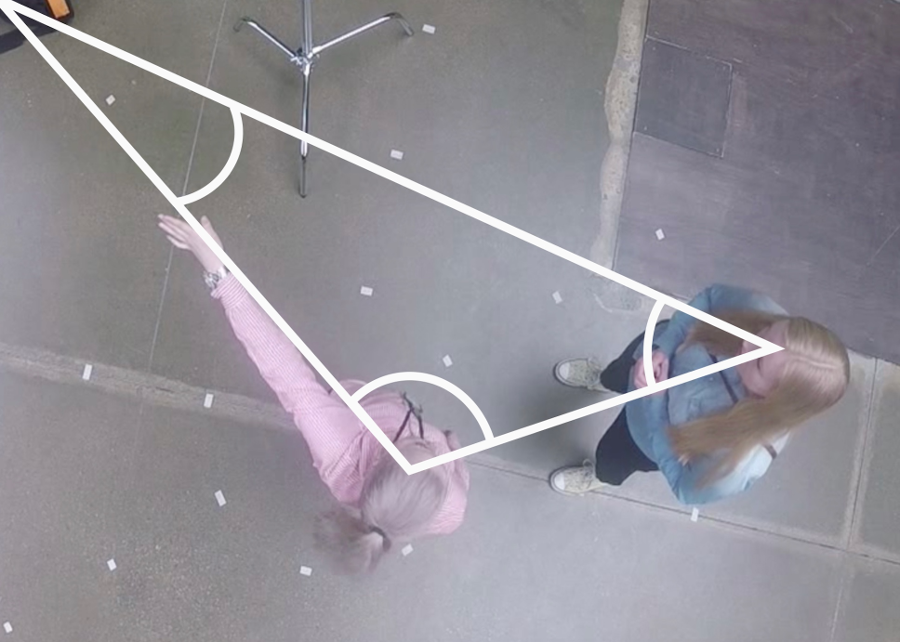
\includegraphics[scale=0.40]{figures/chapter8/human_guide.png}
\caption{\label{fig:chap8_human_guide} Picture from the second Human-Human study \cite{belhassein_2017_human}. Here, the guide is giving the route description to reach a given shop by pointing at it. The formation formed by the guide, the customer, and the target was analyzed. }
\end{figure}

A second exploratory study was then carried out to focus on more complex situations. Among them, we can note situations with two customers requesting directions simultaneously, a customer requesting for two shops at the time, or someone interrupting an ongoing interaction. Once again the formations formed by the guide, the customer, and the landmark were analyzed. An example of such a formation seen during the study can be seen in figure~\ref{fig:chap8_human_guide}. The full results can be found in~\cite{Heikkilae_2018_where} and~\cite{heikkilae_2019_should}. Among these results, the study has shown that the guide usually points to the general location of the target first and in a second step explains and points the different stages of the route.

\section{The deliberative architecture}

In this section, we present the robotic architecture developed to handle the direction-giving task. This architecture relates to Beliefs, Desires, Intentions (BDI) architectures. As explain by~\cite{wooldridge_1999_intelligent}, such a kind of architecture is primarily focused on practical reasoning, meaning the process of deciding step by step which action to perform to reach a goal. 

\begin{figure}[ht!]
\centering
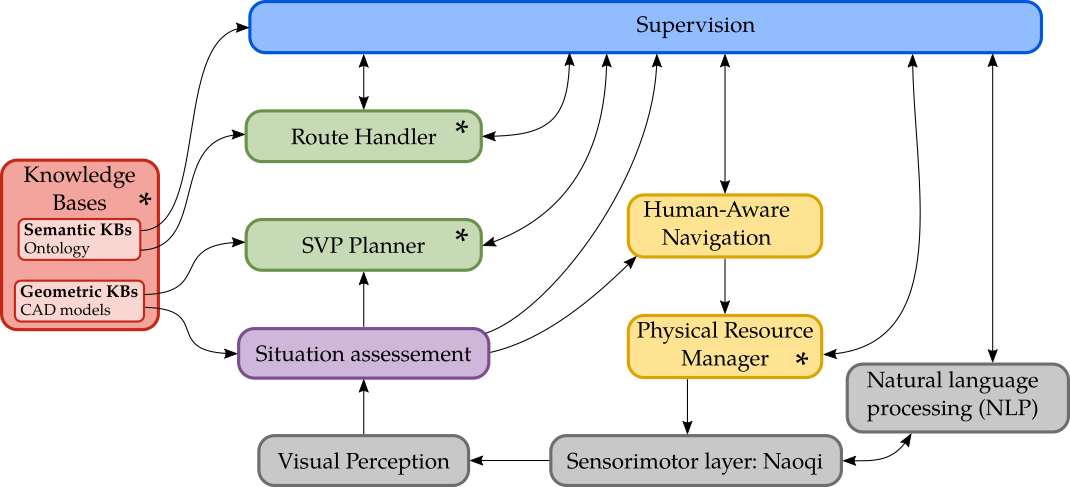
\includegraphics[width=\textwidth]{figures/chapter8/architecture.png}
\caption{\label{fig:chap8_architecture} The general architecture developed for the robot guide. The components presented in this chapter are the colored blocks. The red components with the symbol * are the ones on which I participate. The visual perception and dialogue components have been respectively developed by IDIAP and HWU and are described by~\cite{foster_2019_mummer}. Naoqi is a Softbank Robotics software. }
\end{figure}

The figure~\ref{fig:chap8_architecture} represents the architecture, its components, and their interconnections. Communication between components relies on ROS. In this chapter, we only present the components developed by the LAAS-RIS team, represented by the colored blocks on the architecture. First, we present the two knowledge representations in the form of geometric and semantic representations. Next, we introduce the components related to the sensorimotor layer. It is the situation assessment and the physical resource manager. Then, we present the components related to the deliberative layer. They are the Human-Aware Navigation, the SVP (Shared Visual Perspective) planner, the Route Handler, and finally, the one linking all the components, the Supervision. The Route Handler, part of the deliberative layer, having been presented in detail in chapter~\ref{chap:3}, will not be detailed in this chapter.

\subsection{Environment representation}

For a service robot providing directions to people, we need information to understand humans' need, information to compute the route to the goal, and information to compute the visibility of both agents to plan the pointing position. To understand the needs of a human wanted to be guided, we need information about the type of stores and the sold items. To provide so, \cite{satake_2015_field, satake_2015_should} used an ontology. To compute the route to the final destination, \cite{matsumoto_2012_you} or \cite{okuno_2009_providing} used a topological map. Each node of the graph is related to a 2D position of the environment. To estimate the human visibility of elements anywhere in the environment, \cite{matsumoto_2012_you} used a simplified 3D model where shops are represented by 3D polygons. In our implementation, we only used two types of representation of the environment: a \textbf{geometric} and a \textbf{semantic}.

Since the final deployment of the robot was in a Finland mall, we have built an mockup mall in our lab for development purposes. By mockup, we mean that shops signs have been displayed in the laboratory to create configuration similar to the real mall. The representations describe hereafter have thus been created both for the real mall and the mockup one.

\subsubsection{Geometric representation}

The geometric representation is used to compute the visibility of elements of the environment from different positions needed for the pointing of landmarks. However, because the robot does not accompany the person to the final destination and therefore does not move much, the possible visibility of the two agents is limited to their immediate environment. For this reason and due to the large scale of the Finland mall, we chose to geometrically describe only the subpart of the global environment that could be visible from the interaction area. For the rest of the environment, we represented the shops with 3D points only. These points are enough to point in the right direction. The resulting geometrical representation is a three-dimensional mesh model, as shown in figure.~\ref{fig:chap8_adream_base} for the mockup mall and in figure~\ref{fig:chap8_ideapark_base} for the real one. We have represented in the 3D model all the elements that could hinder visibility, such as poles or panels. In this way, we can precisely emulate human visibility. The model was created from the architectural plans first and then refined with measurements in the mall.

\begin{figure}[ht!]
\centering
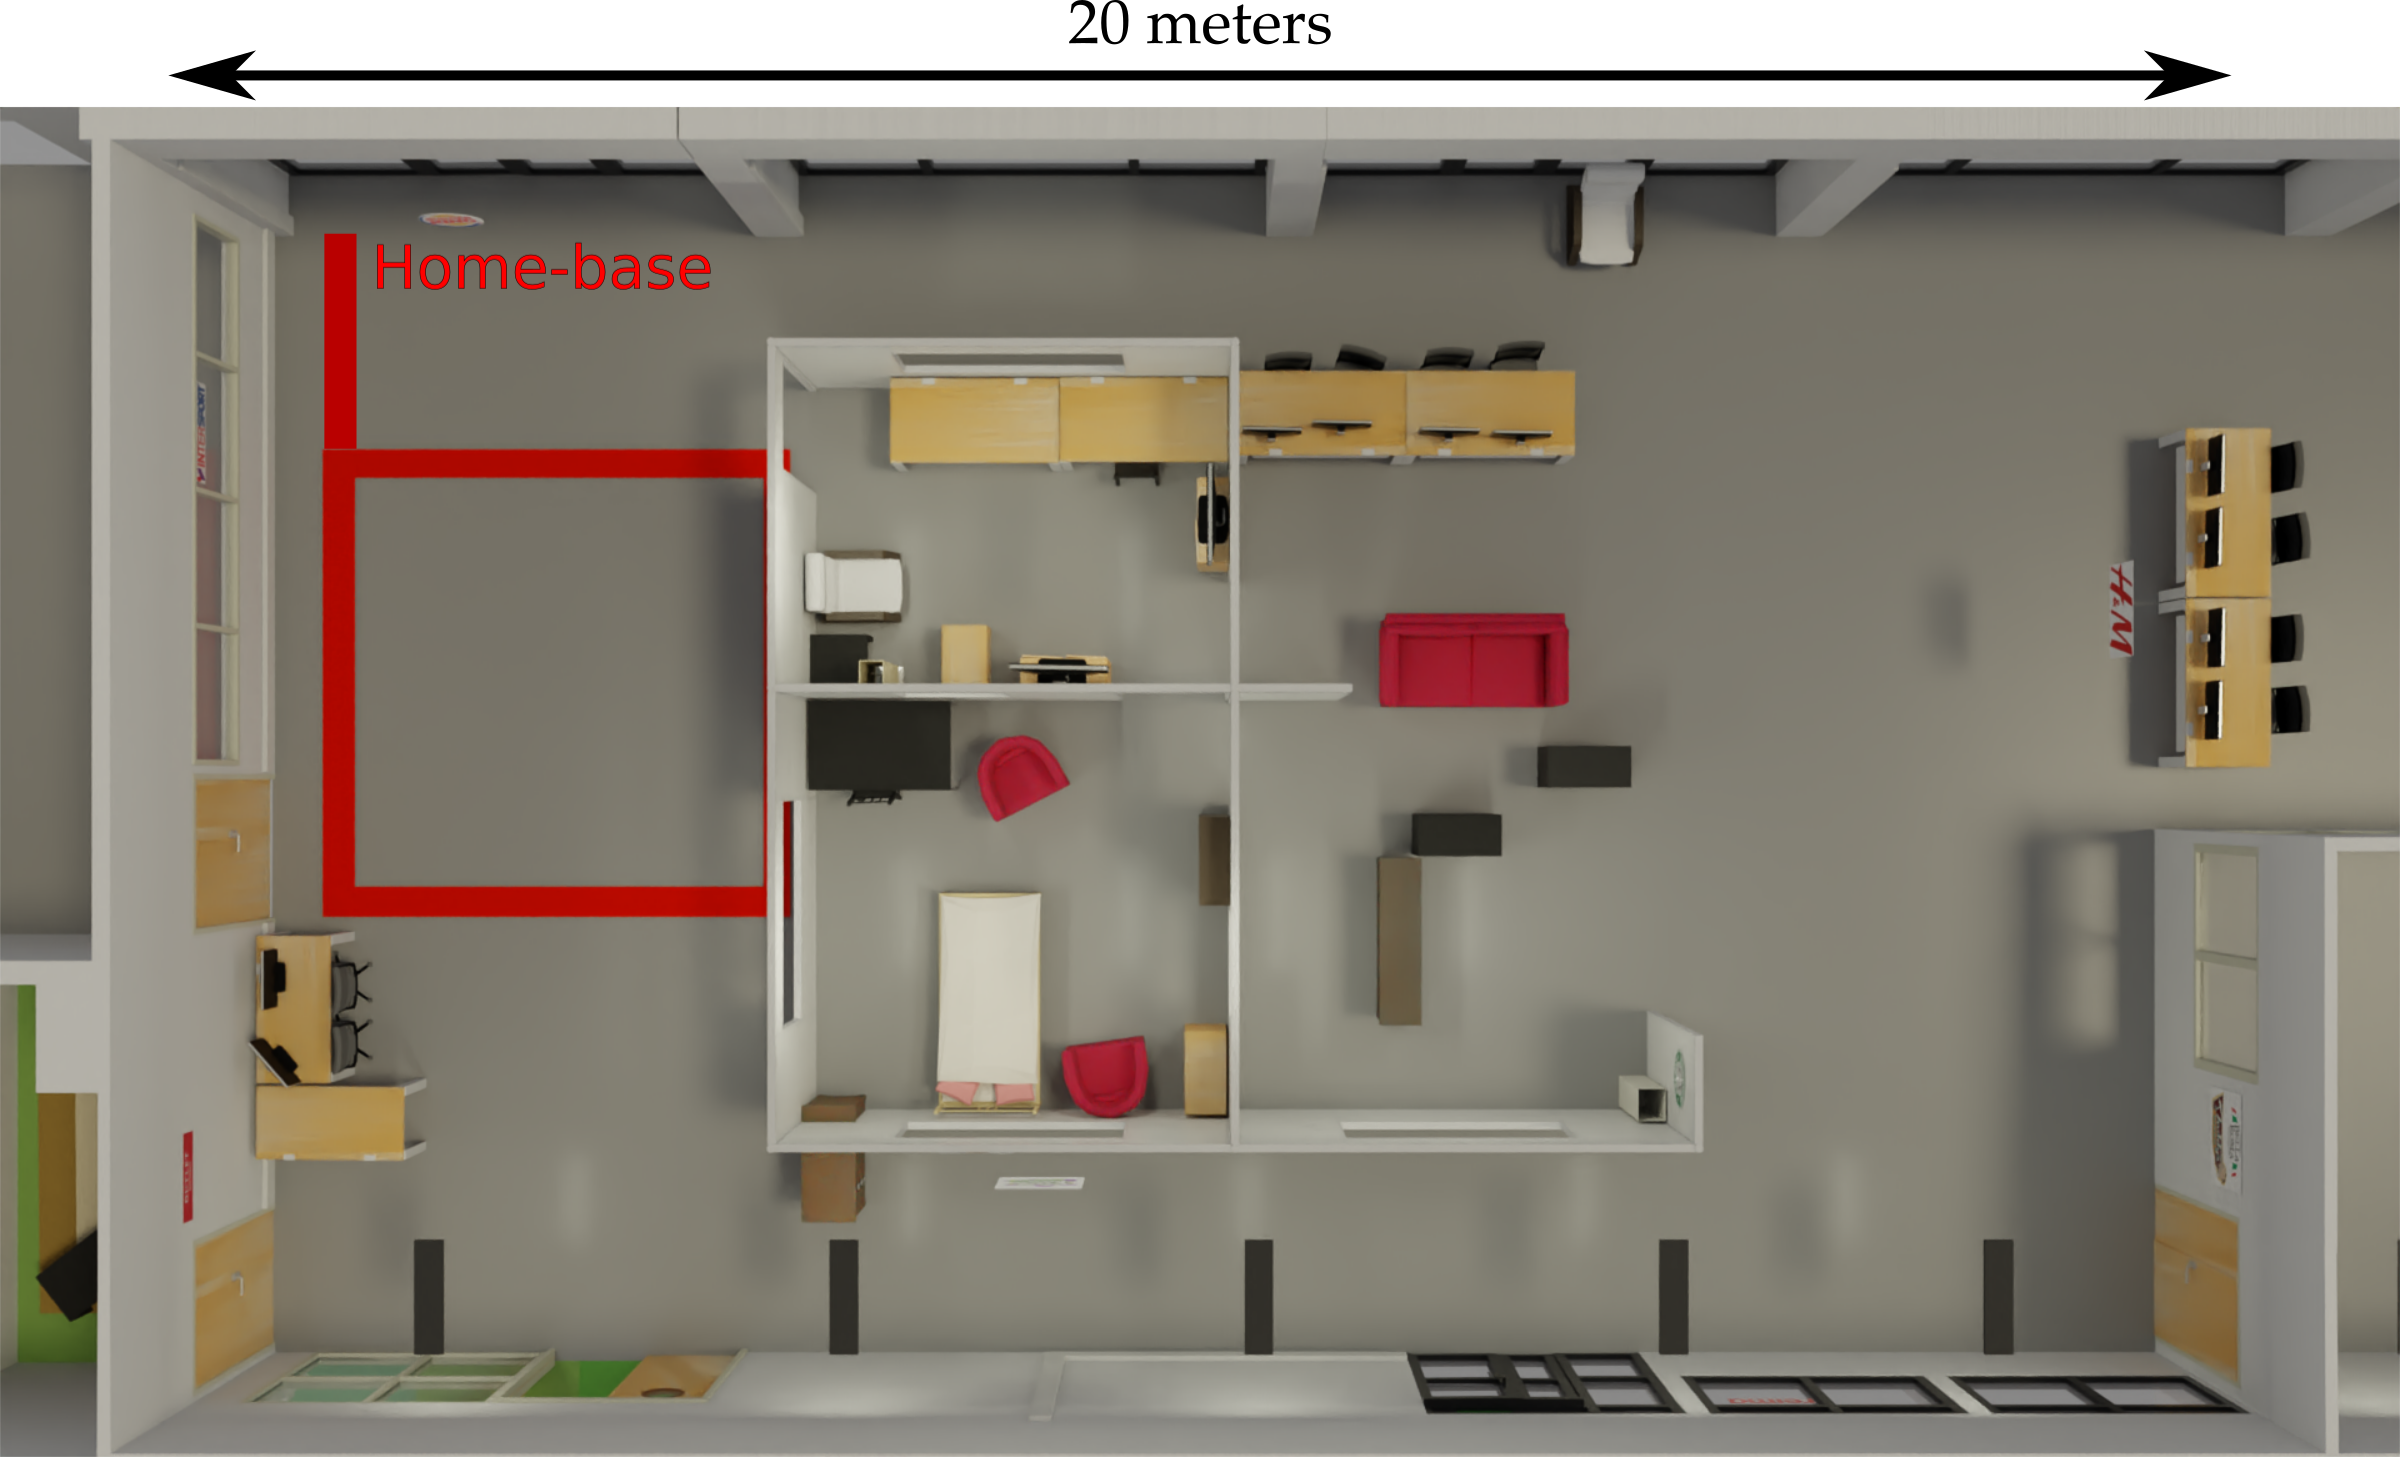
\includegraphics[scale=0.15]{figures/chapter8/adream_base_m.png}
\caption{\label{fig:chap8_adream_base} The 3D mesh model of the mockup mall at laboratory. The red square represent the interaction area as a square of 4 meters per 4 meters. Signs representing the shops have been place all around the environment. }
\end{figure}

\begin{figure}[ht!]
\centering
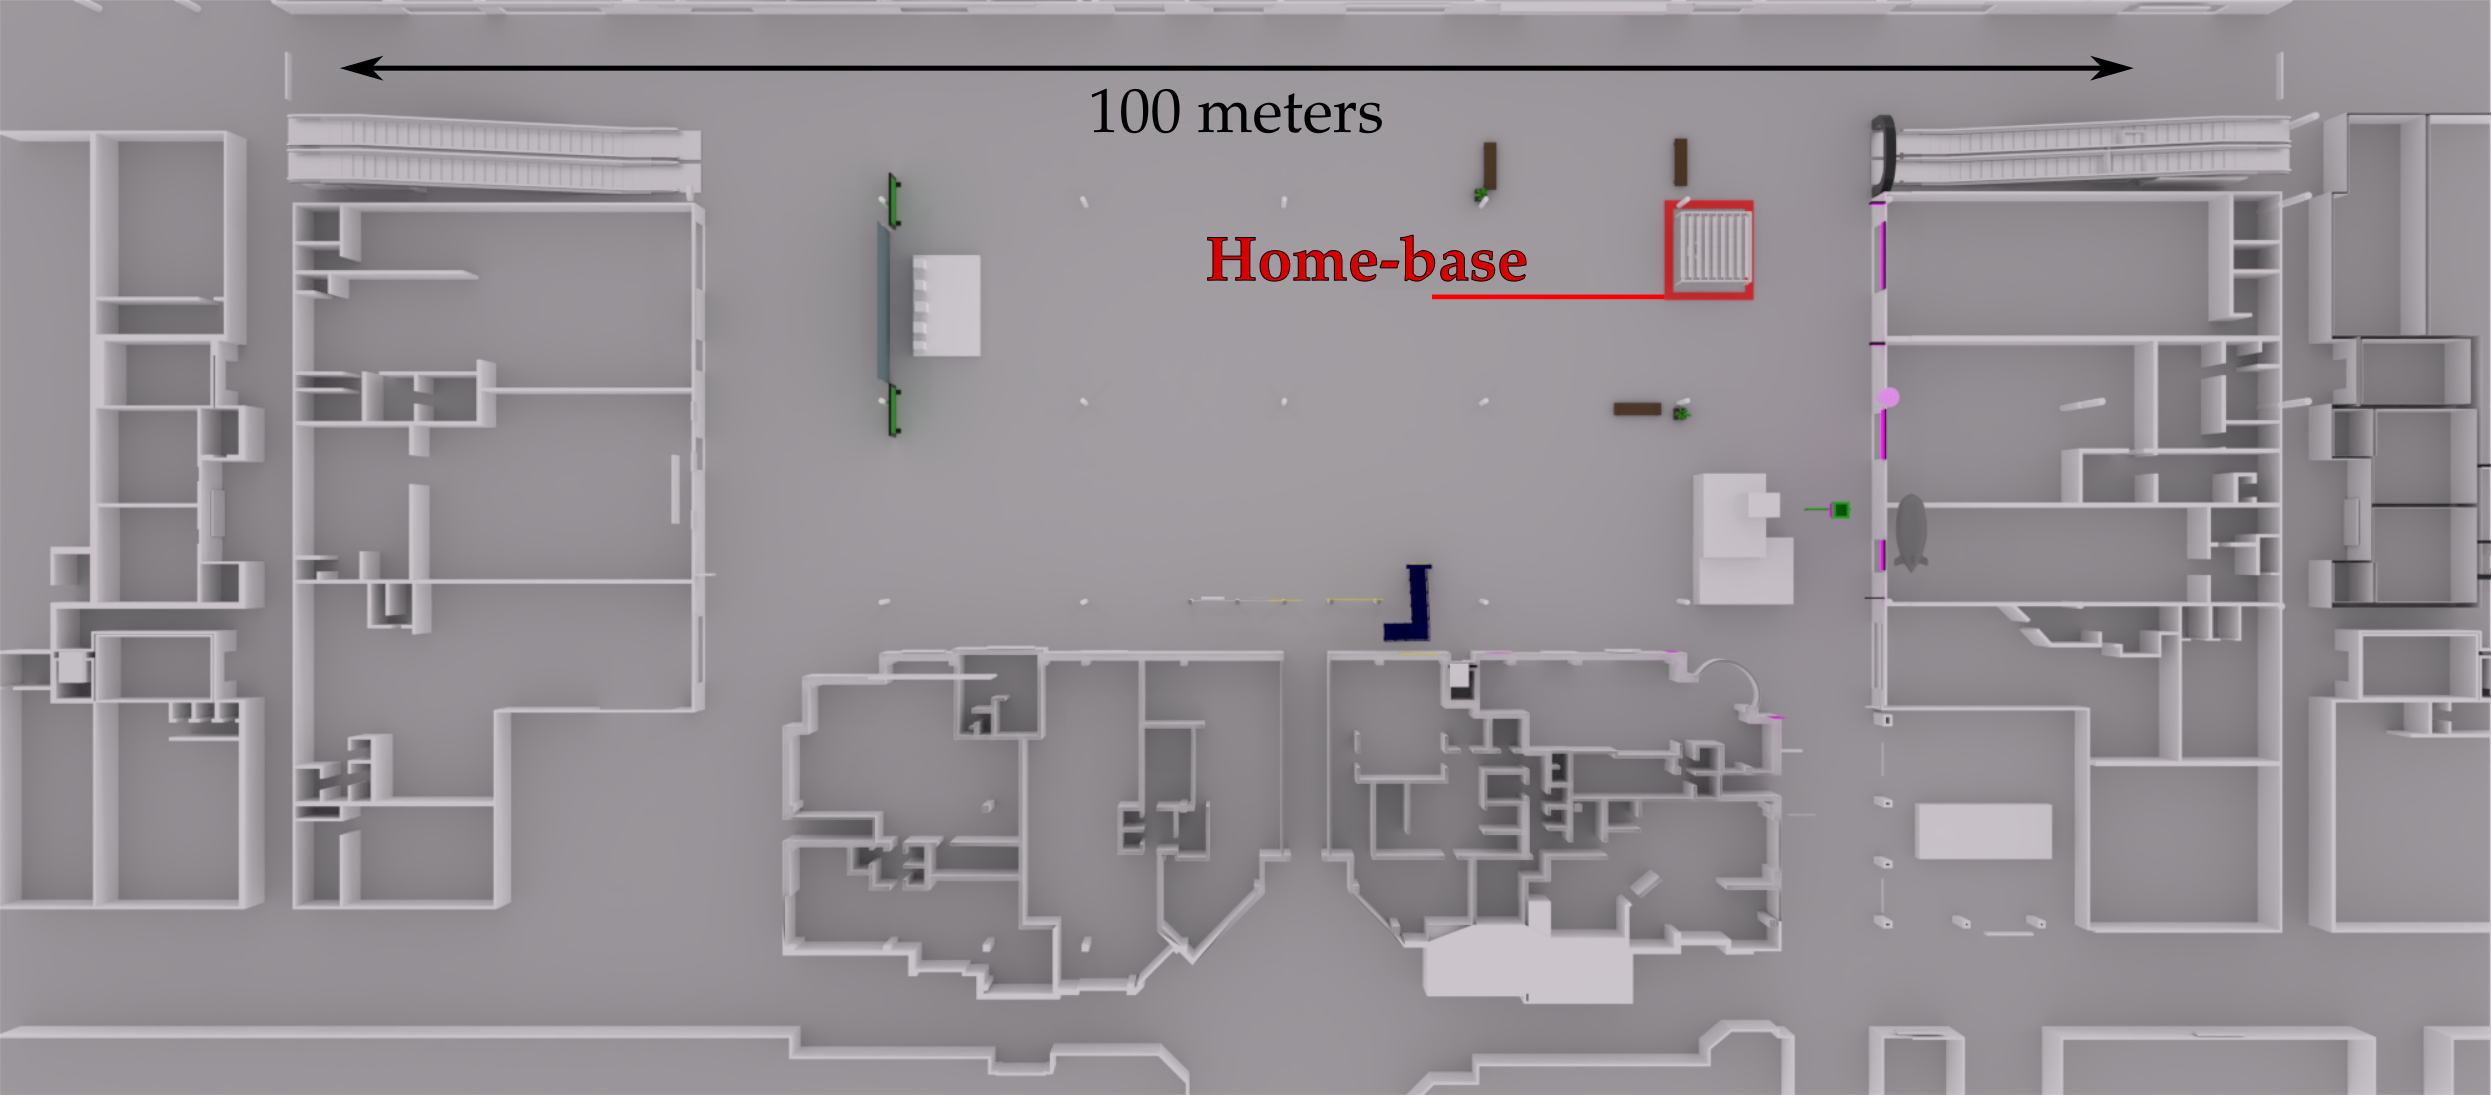
\includegraphics[scale=0.15]{figures/chapter8/ideapark_base_m.png}
\caption{\label{fig:chap8_ideapark_base} The 3D mesh model of the real mall in Finland. The entire mall having a size of 528.6 meters per 247.5 meters on two levels, we have only modelled the part which can be visible from the interaction area. It results in a model of 150 meters per 69 meters. }
\end{figure}

In order for the pointing planner to compute the visibility of the landmarks used for the route description, stairs, escalators, elevators, and store signs are represented each by a single mesh while the rest of the building is a unique 3D mesh. This means that a store is said to be visible if we can see its sign, which we think to be the most relevant element to see to recognize a shop.

The 3D model is also used to generate a navigation map, constraining the robot to move in the interaction area while avoiding obstacles in it.

\subsubsection{Semantic representation}

The environment semantic representation is oriented toward communication and human navigation in a mall. It makes use of the terms, affordances and actions that are needed to walk around in the mall. It represents the needed human-robot common ground knowledge and is used by the robot to perform dialog acts concerning shop names and categories a well as the types of products sold.

This representation takes the form of an ontology. It uses the \acrfull{ssr} (see chapter~\ref{chap:3}) to describe the environment topology. The notion of place is then extended to represent information about the stores. It allows to define and refine the shared goal of the task by understanding the client's wanted destination. We thus represented in it the stores' types, their names, and the items they sell with a richer semantic. It allows for example to represent that both soda and hamburgers are sold in fast-foods, which are types of restaurants, but that soda can also be found in a supermarket. Thanks to Ontologenius, the names of concepts are defined in different languages and with synonyms for these names. It allows the robot to adapt itself to the human partner language. Moreover, with Ontologenius, we endow the robot with the ability to recognize a set of names in natural language but that it will be prevented to use. For example, the robot can understand a reference to ``bank'' when a human says it but only refers to it as ``ATM'' or ``cash machine'' since there was no bank office in the mall. In addition, we used the provided fuzzy matching service to help the supervision system to handle ambiguities coming from the speech-to-text component. For example, if the language recognition module catches the word ``Juwelsport'', we can match it with ``Juvesport'', being a shop in the mall. This set of functionalities around the concepts' names facilitates the understanding of the partner's need and thus helps at increasing the quality of interaction.

\begin{figure}[ht!]
\centering
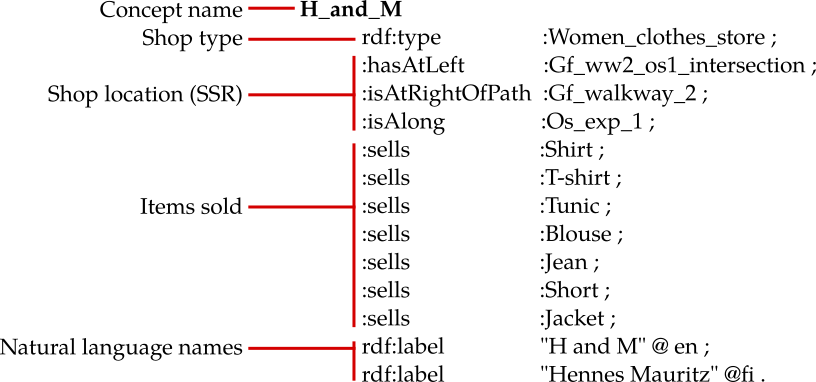
\includegraphics[scale=0.5]{figures/chapter8/zizzi.png}
\caption{\label{fig:chap8_zizzi} Representation of the knowledge about the shop H\&M stored in the ontology. We have both purely semantic knowledge and topological information. }
\end{figure}

An example of the final semantic knowledge represented in the ontology for a given shop is presented in figure.~\ref{fig:chap8_zizzi} for a clothes shop called ``H\&M''. We find in this description the identifier of the shop, the category to which each store belongs, the topological information, the items sold and the names and synonyms in natural language and that for different languages.

\subsection{Perceiving the partner}

The situation assessment component is based on the Underworld framework~\cite{lemaignan_2018_underworlds}. It aims at gathering perception information in the form of 3D position and orientation of human faces, with the 3D model and the robot state. With this information, it is able to generate the symbolics facts listed in table~\ref{tab:chap8_predicates}.

\begin{table}[ht!]
    \centering
    \begin{tabularx}{\textwidth}{|l|X|}
     \hline
    \textbf{Predicate} & \textbf{Description} \\
    \hline
    \hline
        isPerceiving & The robot is perceiving a human \\
        \hline
        isCloseTo & The human is within a distance of 0 to 1 meter of the robot \\
         \hline
        isLookingAt & The human is looking at the robot \\
        \hline
    \hline
        isInArea & The human is in the interaction area \\
        \hline
        isEngagingWith & The human is close to the robot and is looking at it \\
       \hline
    \end{tabularx}
    \caption{Facts computed and monitored during the direction-giving task.}
    \label{tab:chap8_predicates}
\end{table}

\subsection{Managing the robot's resources}

A humanoid robot such as Pepper can be seen as a composition of multiple physical components that can act independently of each other. For the pointing task, we identified four resources: the head, both arms, and the base. At the beginning of the interaction, for example, the head is used to find people to interact with, but later it will be used to track the human with the gaze. Several components could access this resource to perform these actions. However, they do not have a global picture of the ongoing task. In this case, a resource could be used by several components at the time. Consequently, it could lead to task failures.

Moreover, in some cases, several resources have to be used simultaneously to perform a high-level action. To point to a landmark, one arm is selected to point while the other has to be lowered. The base is then rotated if the arm reaches the joint limit to point a target on its back. If at least one of the involved resources is simultaneously used to perform another action, the overall high-level action will fail as the global posture will no more be clear. For example, if the human gets too close to the robot and a component tries to move away from a little, the arm would no more point in the right direction.

Thus, the correct handling of all the resources is critical for performing the task, but it can be cumbersome for a deliberative component, such as the Supervision, to do all the micro-management required. To tackle this issue, we designed a physical resource management system to provide an abstraction of each resource. For each of the identified resources, we instantiated a component called \textbf{Resource Manager (RM)}, having multiple inputs. It is endowed with a low-level decision-making ability allowing it to vote for the next command from a given input to be executed. Its choice is based on events, priorities, and commands importance. Inputs are divided into two types: \textbf{atemporal inputs} and \textbf{finite state machine inputs}. Atemporal inputs are unit overwriting buffers receiving commands which can be run continuously and preempted at any time. Each atemporal input has semantic meaning. For example, the head manager has an atemporal input dedicated to the monitoring of the interacting human. This input thus receives permanently a command to look at the head of the human to be monitored, even if we do not have to look at him. When this input is voted, the robot looks at this point. Finite state machine inputs are prioritized queues of state machines. Each state corresponds to a command to be executed. Transitions can be events received from other components or durations. In this scheme, a state machine cannot be preempted, as it is seen as a set of commands being part of the same high-level action, like a pointing.

To deal with high-level actions requiring multiple resources, we created a \textbf{Resource Synchronizer}. It does not have atemporal inputs but only one finite state machine inputs. It can thus receive finite state machines handling multiple resources, so-called coordination signals. The synchronizer checks if the needed resource managers are free or preemptable, if so, it dispatches the state machines to the proper resource managers and ensures their synchronicity when needed. The synchronizer also reports the status of the ongoing coordination signal to the Supervision component to monitor the progress of the action.
The global resource management scheme is illustrated in figure~\ref{fig:chap8_rm} with four resource managers and one synchronizer.

\begin{figure}[!hb]
\centering
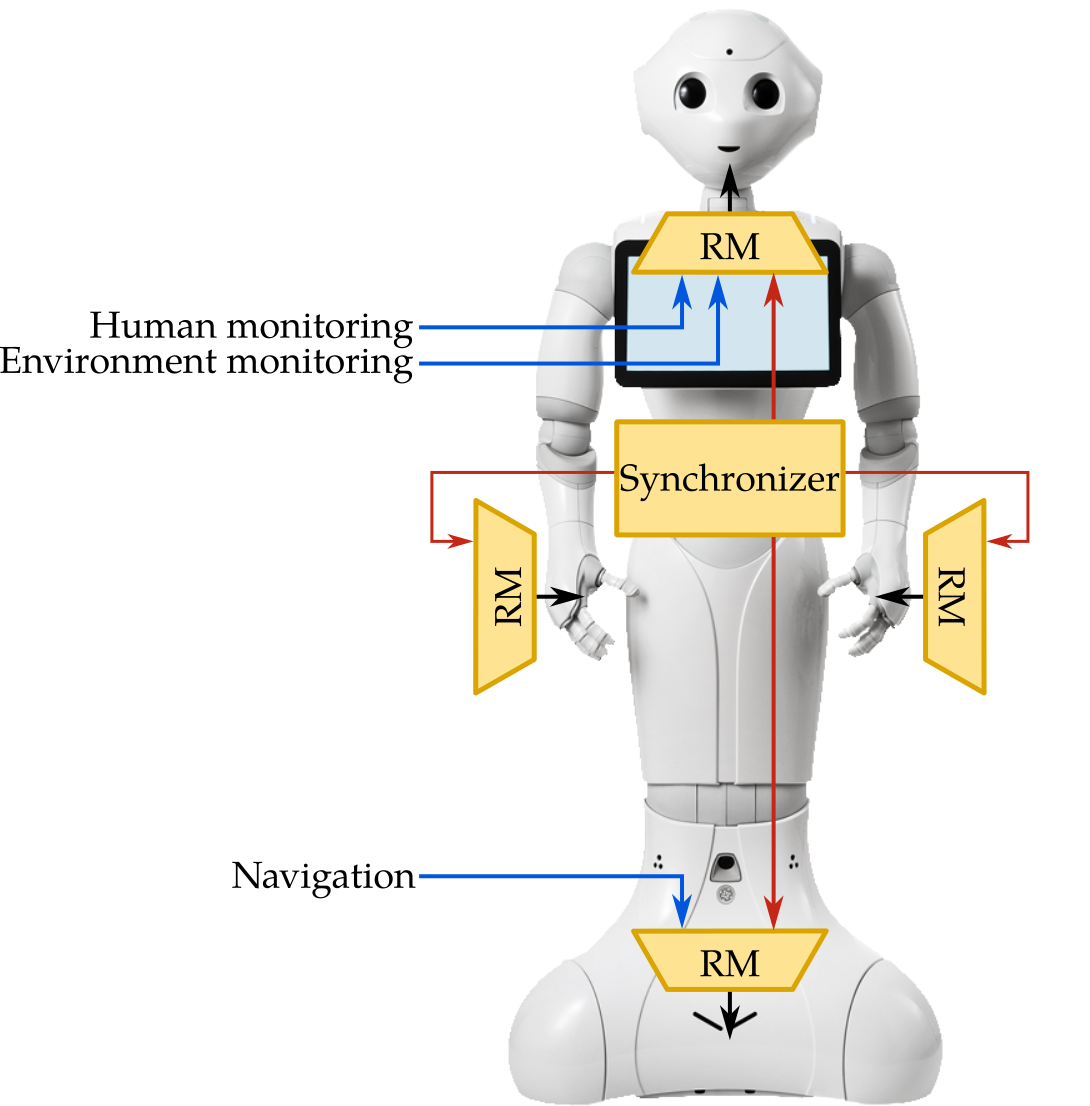
\includegraphics[scale=0.26]{figures/chapter8/rm.png}
\caption{\label{fig:chap8_rm} Representation of the resource management system with four resource managers and a synchronizer. The red arrows represent the state machines inputs and the blue arrows represent the atemporal inputs.}
\end{figure}

\subsection{Describing the route to follow}

The route description process has already be presented in chapter~\ref{chap:3}. However, in the context of the \acrshort{mummer} project, the robot has to be deployed in a Finnish mall. Consequently, the description of the route to follow has to be in Finnish.

The Finnish language is not suitable for pattern-based solutions with placeholders to fill. Indeed, the nouns and verbs have a large number of inflection types, some of which are more common than others. Since it would be too difficult to build sentences as we did for the English version, we chose to generate the explanation in English and then translate it using the Google Translate API. An issue with this solution is that even the names of the stores are translated by giving incorrect sentences. We could think to fill the placeholders after the translation but in some types of sentences, store names would have to be declined. To pass over this later issue, we have limited the variety of sentences to only keep the ones for which it is not necessary to decline store names. This gives less diversity in the way the robot expresses itself but allows more reliable translations. Finally, in some cases, we had to degrade the English quality, creating syntactically incorrect English sentences, so the Finnish translation can be right.

\subsection{Planning a shared visual perspective}

When the robot has to point to a target, two criteria have to be respected. First, the human has to be able to see the target. Second, the human has to be able to look at the pointed target and at the robot without turning the head too much. It goes the same for the robot as it has to see the pointed target, meaning not to point toward a wall and be able to simultaneously point at the target and look at the human. Consequently, to point a target in its back, it has to move. The robot and the human can thus move in the interaction area during the direction-giving task, to move to a better position for pointing at the target. To find the robot and human possible positions we designed a component called the SVP (Shared Visual Perspective) Planner, presented in~\cite{waldhart_2019_reasoning}. For the purpose of the deployment, the presented version is an adapted and slightly simplified version.

To compute the visibility of both agents, the planner has access to the geometrical representation of the environment and the agents current positions. In addition, it considers an estimated agent's maximal speed to move and a visibility threshold.

When the robot explains the route to the human and points to a landmark, they form what is called an F-formation. Kendon explains that \textit{``An F-formation arises whenever two or more people sustain a spatial and orientational relationship in which the space between them is one to which they have equal, direct and exclusive access''} \cite{kendon_1990_conducting}.
This F-formation has been decomposed in \cite{mcneill_2005_gesture} into two types: the social formation and the instrumental formation. While the first type corresponds to the original definition, the instrumental formation includes a physical object that all the agents can gaze at. This means that once the robot will have moved, the human will come in front of it creating a social formation in the form of a vis-a-vis (each facing the other) and when the robot will point they will change for an instrumental formation. Indeed, when both agents will reach their position computed by the planner, we want them to be able to go from one formation to the other with only a rotation; the human will not need to move again from their arriving position to see what the robot will point. 

To search for better positions to reach in order to point a landmark, the planner takes three main parameters into account:

\begin{itemize}
    \item Visibility constraint: The two agents can see either the target shop when it is the only element of the route or the passage.
    \item Navigation distance cost: The agents do not have to move too much.
    \item F-formation cost: The human-robot-target angle and a robot-human-target have to be less than 90${^\circ}$. 
\end{itemize}

\begin{figure}[ht!]
\centering
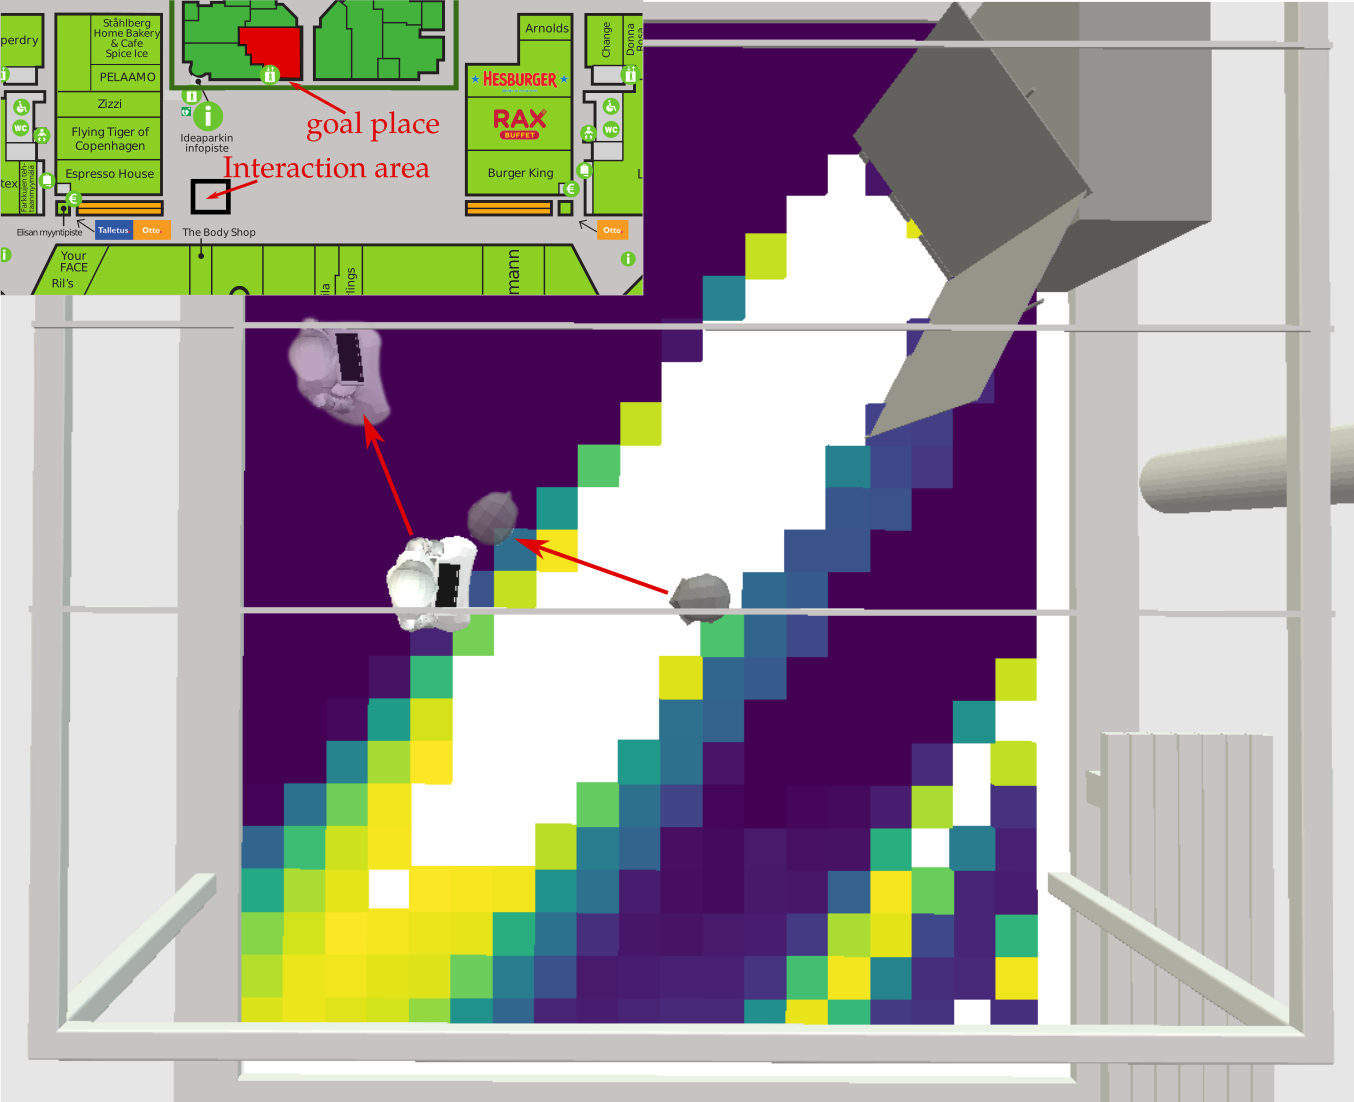
\includegraphics[scale=0.3]{figures/chapter8/grid_map.png}
\caption{\label{fig:chap8_svp_grid} Visibility grid for a target located at the top right. The uncoloured areas represent an absence of visibility and the others represent the cost of visibility ranging from yellow for low visibility to purple for good visibility. The robot and the human in transparency on the image represent the final calculated positions while the others are the initial positions. }
\end{figure}

To compute the positions, the interaction area is firstly decomposed into a weighted three-dimensional (x,y for the possible positions in the area and z for the human height) grid representing the estimated human visibility of the target. The target visibility is computed offline for each position of the grid. It is based on the part that the target takes in the 360${^\circ}$ field of view of the environment. Such grid is represented in figure~\ref{fig:chap8_svp_grid} for a given human height. The white cells are positions from which the human cannot see the pointed target. The other colored cells represent the degree of visibility from the poor in yellow to the good in purple. Having the human visibility grid, the goal position is computed using a weighted cost function between good visibility and restricted distance to cross. In the example of figure~\ref{fig:chap8_svp_grid}, the transparent human head is the human goal position while the other is the initial position. From the initial position, the human was not able to the pointed target.

The overall computation flow is illustrated in figure~\ref{fig:chap8_svp}. The robot position is computed in a second time, according to the human planned position. Divided the search into two steps allows reducing the search complexity. The robot position is thus constrained by the human one. It has also to respect a minimal and maximal distance to the human and minimal visibility of the target from it. Finally, the robot position is also determined regarding a cost preferring an F-formation limiting the robot reorientation, meaning that it can point to the target keeping its torso and its chest oriented towards the human.

\begin{figure}[ht!]
\centering
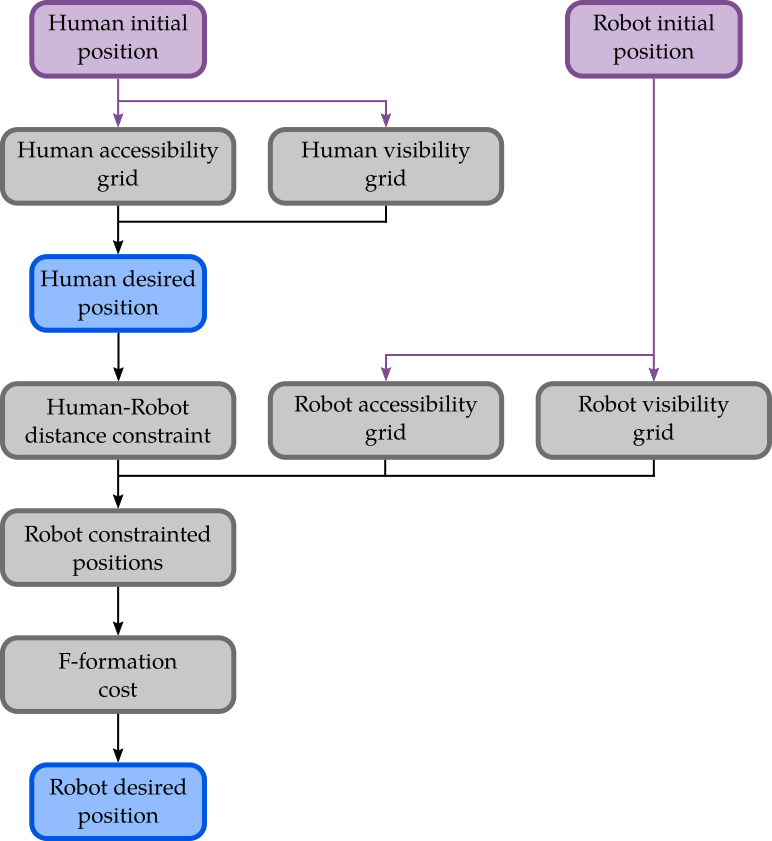
\includegraphics[scale=0.44]{figures/chapter8/svp.png}
\caption{\label{fig:chap8_svp} Human and robot positions computation flow. The purple blocks represent the initial positions while the blue ones represent the planned positions. }
\end{figure}

\subsection{Navigate close to human}

The Human-Aware Navigation component aims at moving the robot while avoiding dynamic and static obstacles in addition to proposing a socially acceptable navigation solution for the robot. For example, the robot should not pass too close to the human and should not show its back while navigating around the human. A full presentation of the planner is available in~\cite{singamaneni_2020_hateb}.

\subsection{Executing and controling the task}

The Supervision component aims at implementing the joint action guidelines to manage the direction-giving task as a human-robot joint activity. It makes use of all the other components of the architecture to step-by-step establish the shared goal, plan by considering the human preferences, adapt to the human perspective of the scene, and monitor human commitment. The action sequencing and the incremental task-refinement process follows the steps and the main decisions exhibited in human-human studies. 

First, when the Supervision receives for example a request for a restaurant from the Dialogue, it asks Ontologenius for all the existing restaurant types. This list of restaurant types is sent to the Dialogue whose role is to return to the Supervision with the type selected by the human. It then continues to obtain a more precise restaurant type from the human to finally get a restaurant name. It goes the same if the human asks for a product. The Supervision gets from Ontologenius a list of shops selling the requested item and passes it to the Dialogue. The Dialogue returns the name of the shop chosen by the person. When it directly receive as a goal a shop name, it queries the ontology to know if the given shop exists in the mall. If it does not, it can be misunderstood. To test it, the Supervision can query the Ontologenius using the fuzzy match feature. For example, when a person asks to go to ``jewelsport'', the system can make the assumption that the person actually asked for ``Juvesport''.

Once the shared goal determined, the Supervision queries the Route Handler which returns a list of routes of the form $place - path - place - ... - place$. Among these routes, it selects the one with fewer elements. If it is composed of only one path, it means that the goal place can be visible from there as being on the same path as the robot. Otherwise, the robot will have to explain the route. Before that, it tests if the route has stairs along with it, getting the types of the elements with the ontology. If so, the supervision is in charge of ensuring the human is able to climb stairs. If he cannot, the supervision selects another route, without stairs.

The robot's role is not only to give verbal route directions but also to point to the target or the passage the person should take. We call the passage the third element of the route. It is the first element the human has to go through to start the route\footnote{The first element of the route returned by Route Handler is their current location.}. Pointing increases the chances to find the destination as it helps to orient oneself in space. Before pointing, the supervision requests the SVP planner for a new position for itself and the human. If the current positions do not fit the visibility and formation constraints, the supervision uses the Human-Aware navigation module to go to its new position. We expect the human to come in front of it. If he does not, the supervision is able to verbally inform him about movements to do (i.e. to come in front of it, to move a bit aside, etc).

Finally, once the human is at the desired position, the supervision requests the Physical Resource Manager for pointing and simultaneously explains the route to take.

In addition to the management of the direction-giving task itself, the supervision component is also in charge of the beginning of the interaction, the greeting, and its end, the goodbyes. All along with the interaction, it also ensures the human understanding of the instructions, and adapt itself if needed.

\section{Embody architecture in a physical robot}

The architecture presented in the previous chapter has been embedded in an upgraded, custom version, of the Pepper platform~\cite{caniot_2020_adapted}, which is equipped with an Intel D435 camera and an NVIDIA Jetson TX2. It has been deployed multiple times in a mall in Finland, Ideapark.

\subsection{Pepper in Ideapark}

For availability for as many customers as possible, the robot was contained in a defined place in the mall as shown in figure~\ref{fig:chap8_pepper_mall}. A home base was designed with the participation of all the project partners. It was a 4 per 4 meters area with a 2.5m high frame structure on it. The home base included a non-reflecting carpet on the floor and an acoustic ceiling surface on the roof.

\begin{figure}[ht!]
\centering
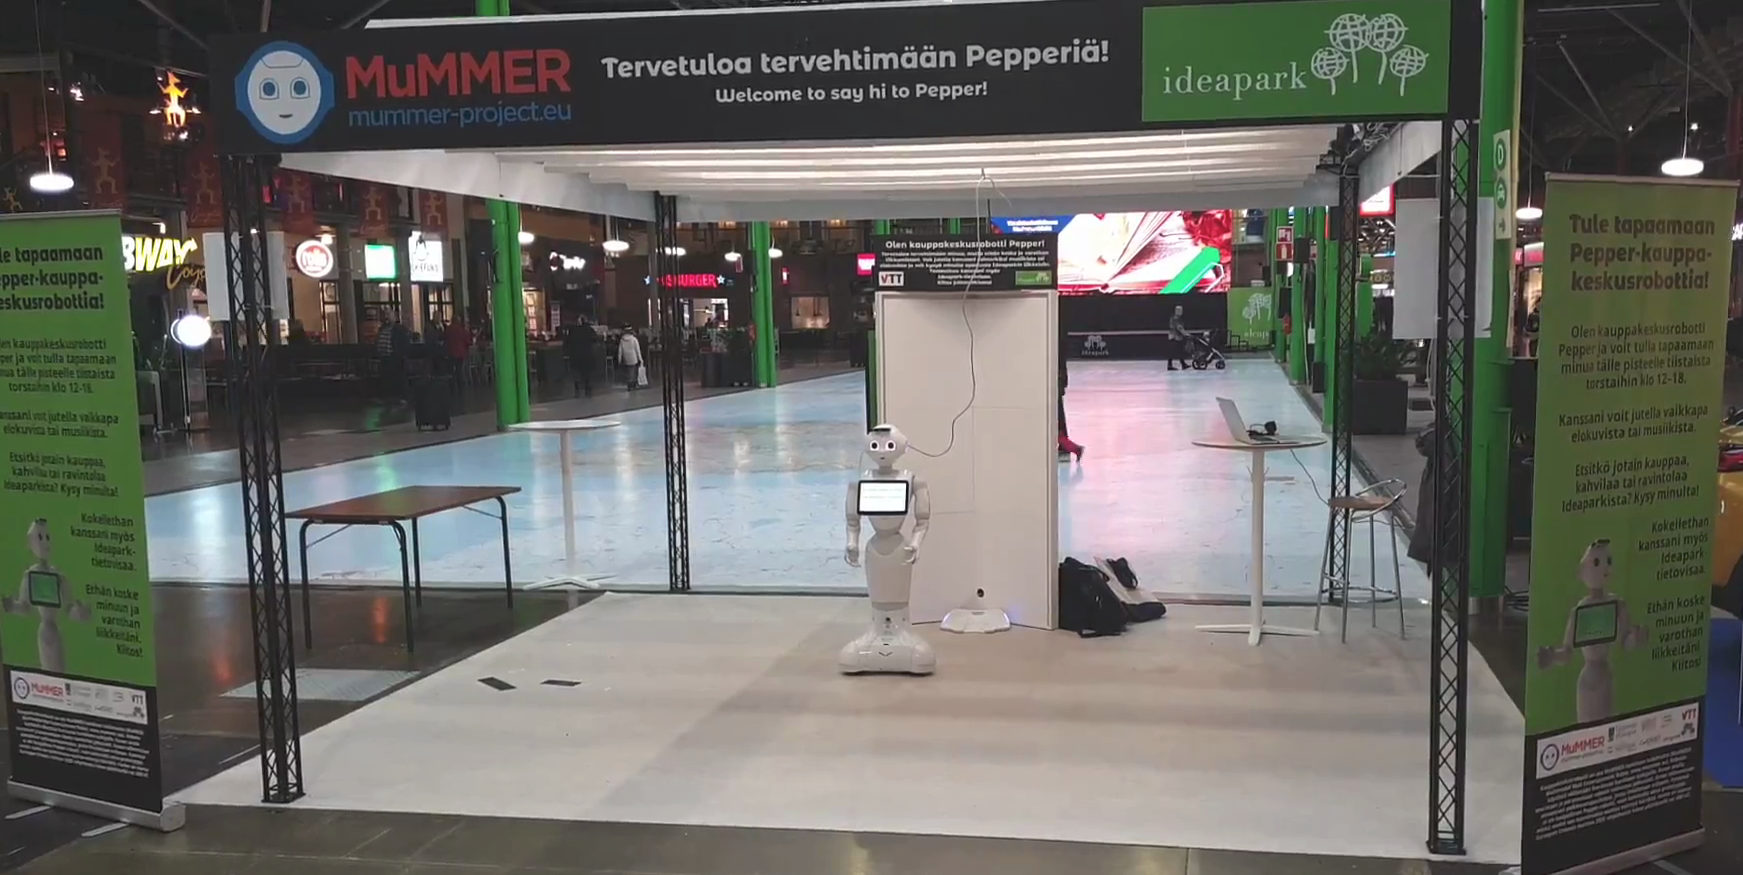
\includegraphics[scale=0.2]{figures/chapter8/pepper_mall.png}
\caption{\label{fig:chap8_pepper_mall} The pepper robot in its interaction area in the Finalnd mall, Ideapark. }
\end{figure}

During the first deployment in the real mall, we have updated both the Geometric Representation with actual measurements and the \acrfull{ssr} by making sure the regions, interfaces, corridors and intersections were represented reflecting the actual mall topology. To ensure the correctness of the instructions given by the route handler, we generated routes from the deployment location to several shops in the mall and followed them to the destination. Inaccuracies, as well as algorithmic flaws, have been fixed using this method. We also tested the interaction in the Finnish language with our native Finnish partners and corrected some mistakes in the route verbalization.

\subsection{Pepper ``in the wild''}

The robot was then installed for a long-term 14 weeks deployment from September 2019 to December 2019. During this period, the robot interacted with everyday clients of the mall, who may never have the chance to interact with a robot before. The robot was active for 3 hours per day, three days a week. In total, the robot ran the direction-giving task for approximately 96 hours ``in the wild''. Out of these 96 hours, it was interacting with customers for 45 hours.
